% Created 2018-04-02 Mon 13:45
% Intended LaTeX compiler: pdflatex
\documentclass[final]{beamer}
	         \usetheme{ph}
           \usepackage[orientation=portrait,size=a0,scale=1.4]{beamerposter}
           \usepackage[absolute,overlay]{textpos}
	         \usepackage[authoryear]{natbib}


\setlength{\paperwidth}{36in}
\setlength{\paperheight}{48in}
\setlength{\textwidth}{0.98\paperwidth}
\setlength{\textheight}{0.98\paperheight}
\graphicspath{{../output/figures/}{../lib/}}
\usepackage[export]{adjustbox}
\usepackage{graphicx,caption}
\usepackage{minted}
\usepackage{eurosym}
\usepackage{listings}
\usepackage{textcomp}
\usepackage{bibentry}
\date{}
\author{
Philipp Homan$^{1}$,
\\
\normalsize{$^{1}$Department of Psychiatry,}
\normalsize{The Donald and Barbara Zucker}
\normalsize{School of Medicine at Northwell/Hofstra,}
\normalsize{Hempstead, NY}
}
\usetheme{default}
\date{2018-04-02 13:45}
\title{A scientific poster entirely written in org-mode using GNU emacs and the beamer library}
\begin{document}

\begin{frame}[fragile,label={sec:org81c45e2}]{}
 \begin{columns}
\begin{column}[t]{0.45\columnwidth}
\begin{block}{Background}
\begin{itemize}
\item Org-mode is not only useful for producing blog posts and even
scientific manuscripts; it is also perfectly suitable to make 
decent looking scientific posters
\item We combine a relatively simple custom \LaTeX style file and common
org-mode syntax
\item The nice thing about org-mode is that we can populate the poster with
code, graphs and numbers from inline code in languages such as R,
python, Matlab and even shell scripting
\item Inline code would look like this, which will produce a graph
(Fig. \ref{fig:org22c0db4}):
\end{itemize}

\begin{columns}
\begin{column}[T]{0.48\columnwidth}
\begin{verbatim}
x <- rnorm(100, 0, 1)
hist(x, col="gray")
\end{verbatim}


\begin{figure}[htbp]
\centering
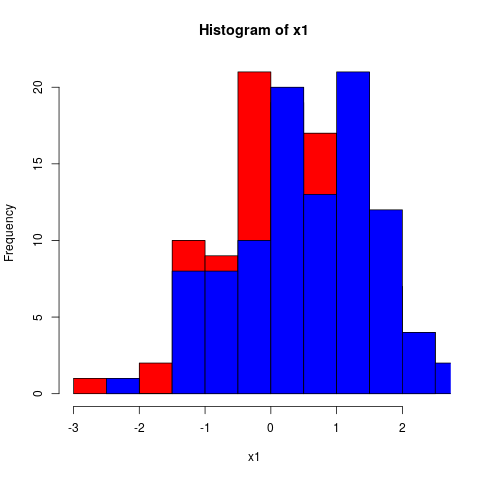
\includegraphics[width=.9\linewidth]{3.png}
\caption{\label{fig:org22c0db4}
This is the output.}
\end{figure}
\end{column}
\end{columns}
\end{block}

\begin{block}{Methods: Inline code and tables}
\begin{itemize}
\item In addition to inline code, we can also produce tables
\item Tables are very powerful in org-mode, they even include spreadsheet
capabilities
\item Some code to process the vector from above to make a table out of its
summary could look like this, which would result in a little table
(Table \ref{tab:org8233f27}) :
\end{itemize}

\begin{columns}
\begin{column}[T]{0.48\columnwidth}
\begin{verbatim}
m <- round(mean(x), 2)
s <- round(sd(x), 2)
data.frame(Mean=m, SD=s)
\end{verbatim}

\vspace{2cm}

\begin{table}[htbp]
\centering
\begin{tabular}{rr}
Mean & SD\\
\hline
-0.06 & 0.94\\
\end{tabular}
\caption{\label{tab:org8233f27}
A table.}

\end{table}
\end{column}
\end{columns}
\end{block}
\end{column}



\begin{column}[t]{0.45\columnwidth}
\begin{block}{Results: graphics}
\begin{itemize}
\item Of course we can also include graphics
\item Here, we use shell scripting to grab an image with curl from the
internet (Fig. \ref{fig:org5d9dd5a}):
\end{itemize}

\begin{columns}
\begin{column}[T]{0.78\columnwidth}
\small
\begin{verbatim}
curl -0 https://www.gnu.org/software/emacs/images/emacs.png
\end{verbatim}
\normalsize

\vspace{2cm}

\begin{figure}[htbp]
\centering

\includegraphics[page=9,width=0.2\textwidth]{emacs.png}
\caption{\label{fig:org5d9dd5a}
This is the downloaded image.}
\end{figure}
\end{column}
\end{columns}
\end{block}

\begin{block}{Results: columns}
\begin{columns}
\begin{column}[T]{0.48\columnwidth}
\captionsetup{justification=justified,width=.8\linewidth}
\begin{figure}[htbp]
\centering

\includegraphics[page=3,width=0.9\textwidth]{org-mode-poster-4.png}
\caption{\label{fig:orgae102b5}
\textbf{This is the left figure of a two-column block}}
\end{figure}
\end{column}

\begin{column}[T]{0.48\columnwidth}
\captionsetup{justification=justified,width=.8\linewidth}
\begin{figure}[htbp]
\centering

\includegraphics[page=9,width=0.9\textwidth]{org-mode-poster-4.png}
\caption{\label{fig:org5e6c798}
\textbf{This is the right figure.}}
\end{figure}
\end{column}
\end{columns}
\end{block}

\begin{block}{Conclusions}
\begin{itemize}
\item This little example is meant to show how incredibly versatile
org-mode is
\item One can now produce scientific posters with a simple text editor
\end{itemize}
\end{block}
\end{column}
\end{columns}
\end{frame}
\end{document}
